\documentclass{standalone}
\usepackage{tikz}
\usetikzlibrary{patterns, positioning}


\begin{document}
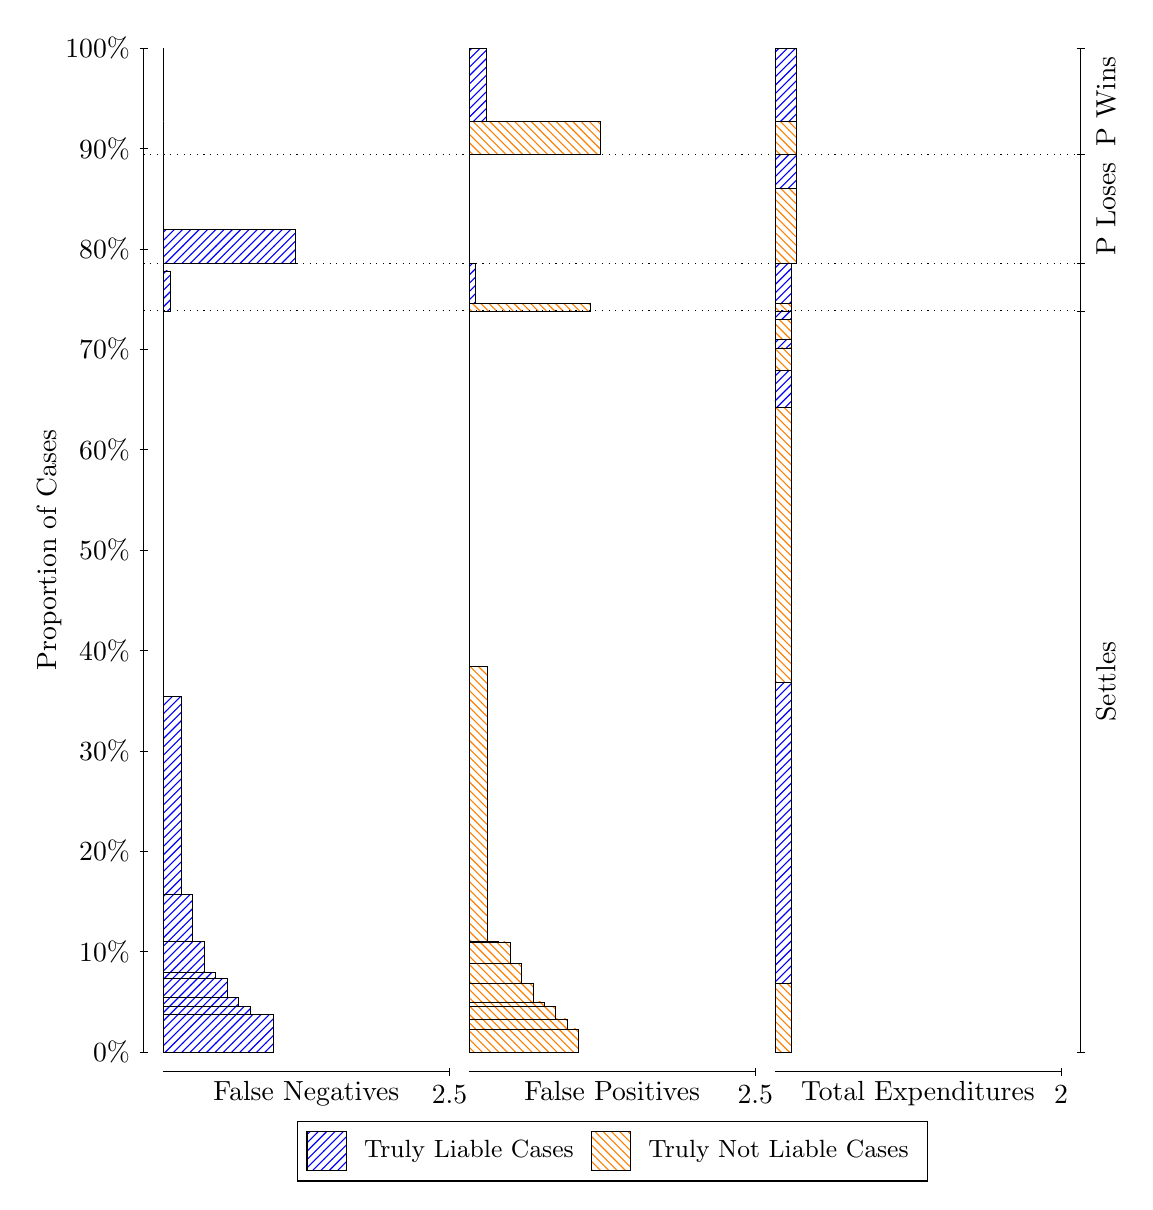
\begin{tikzpicture}
\draw[black, very thin] (1.5,1.75) -- (1.5,14.5);
\node[rotate=90, text=black, anchor=center] at (0.3, 8.125) {Proportion of Cases};
\draw[black, very thin] (1.45,1.75) -- (1.55,1.75);
\node[text=black, anchor=east] at (1.45, 1.75) {0\%};
\draw[black, very thin] (1.45,3.025) -- (1.55,3.025);
\node[text=black, anchor=east] at (1.45, 3.025) {10\%};
\draw[black, very thin] (1.45,4.3) -- (1.55,4.3);
\node[text=black, anchor=east] at (1.45, 4.3) {20\%};
\draw[black, very thin] (1.45,5.575) -- (1.55,5.575);
\node[text=black, anchor=east] at (1.45, 5.575) {30\%};
\draw[black, very thin] (1.45,6.85) -- (1.55,6.85);
\node[text=black, anchor=east] at (1.45, 6.85) {40\%};
\draw[black, very thin] (1.45,8.125) -- (1.55,8.125);
\node[text=black, anchor=east] at (1.45, 8.125) {50\%};
\draw[black, very thin] (1.45,9.4) -- (1.55,9.4);
\node[text=black, anchor=east] at (1.45, 9.4) {60\%};
\draw[black, very thin] (1.45,10.675) -- (1.55,10.675);
\node[text=black, anchor=east] at (1.45, 10.675) {70\%};
\draw[black, very thin] (1.45,11.95) -- (1.55,11.95);
\node[text=black, anchor=east] at (1.45, 11.95) {80\%};
\draw[black, very thin] (1.45,13.225) -- (1.55,13.225);
\node[text=black, anchor=east] at (1.45, 13.225) {90\%};
\draw[black, very thin] (1.45,14.5) -- (1.55,14.5);
\node[text=black, anchor=east] at (1.45, 14.5) {100\%};

\draw[black, very thin] (13.4,1.75) -- (13.4,14.5);
\draw[black, very thin] (13.35,1.75) -- (13.45,1.75);
\node[anchor=west] at (13.35, 1.75) {};
\draw[black, very thin] (13.35,11.162) -- (13.45,11.162);
\node[anchor=west] at (13.35, 11.162) {};
\draw[black, very thin] (13.35,11.768) -- (13.45,11.768);
\node[anchor=west] at (13.35, 11.768) {};
\draw[black, very thin] (13.35,13.145) -- (13.45,13.145);
\node[anchor=west] at (13.35, 13.145) {};
\draw[black, very thin] (13.35,14.5) -- (13.45,14.5);
\node[anchor=west] at (13.35, 14.5) {};

\draw[black, very thin, pattern color=blue, pattern=north east lines] (1.75,1.75) rectangle (3.1398,2.2235);
\draw[black, very thin, pattern color=blue, pattern=north east lines] (1.75,2.2235) rectangle (2.9944,2.2317);
\draw[black, very thin, pattern color=blue, pattern=north east lines] (1.75,2.2317) rectangle (2.8491,2.3329);
\draw[black, very thin, pattern color=blue, pattern=north east lines] (1.75,2.3329) rectangle (2.7037,2.4384);
\draw[black, very thin, pattern color=blue, pattern=north east lines] (1.75,2.4384) rectangle (2.5584,2.6886);
\draw[black, very thin, pattern color=blue, pattern=north east lines] (1.75,2.6886) rectangle (2.4131,2.764);
\draw[black, very thin, pattern color=blue, pattern=north east lines] (1.75,2.764) rectangle (2.2678,3.1502);
\draw[black, very thin, pattern color=blue, pattern=north east lines] (1.75,3.1502) rectangle (2.1224,3.753);
\draw[black, very thin, pattern color=blue, pattern=north east lines] (1.75,3.753) rectangle (1.9771,6.2614);
\draw[black, very thin, pattern color=orange, pattern=north west lines] (1.75,6.2614) rectangle (1.75,11.162);
\draw[black, very thin, pattern color=blue, pattern=north east lines] (1.75,11.162) rectangle (1.8318,11.67);
\draw[black, very thin, pattern color=orange, pattern=north west lines] (1.75,11.67) rectangle (1.75,11.768);
\draw[black, very thin, pattern color=blue, pattern=north east lines] (1.75,11.768) rectangle (3.4213,12.194);
\draw[black, very thin, pattern color=orange, pattern=north west lines] (1.75,12.194) rectangle (1.75,13.145);
\draw[black, very thin, pattern color=orange, pattern=north west lines] (1.75,13.145) rectangle (1.75,13.57);
\draw[black, very thin, pattern color=blue, pattern=north east lines] (1.75,13.57) rectangle (1.75,14.5);
\draw[black, very thin, pattern color=orange, pattern=north west lines] (5.6333,1.75) rectangle (7.0231,2.0445);
\draw[black, very thin, pattern color=orange, pattern=north west lines] (5.6333,2.0445) rectangle (6.8777,2.1704);
\draw[black, very thin, pattern color=orange, pattern=north west lines] (5.6333,2.1704) rectangle (6.7324,2.3259);
\draw[black, very thin, pattern color=orange, pattern=north west lines] (5.6333,2.3259) rectangle (6.5871,2.3852);
\draw[black, very thin, pattern color=orange, pattern=north west lines] (5.6333,2.3852) rectangle (6.4417,2.6192);
\draw[black, very thin, pattern color=orange, pattern=north west lines] (5.6333,2.6192) rectangle (6.2964,2.8733);
\draw[black, very thin, pattern color=orange, pattern=north west lines] (5.6333,2.8733) rectangle (6.1511,3.1475);
\draw[black, very thin, pattern color=orange, pattern=north west lines] (5.6333,3.1475) rectangle (6.0057,3.1575);
\draw[black, very thin, pattern color=orange, pattern=north west lines] (5.6333,3.1575) rectangle (5.8604,6.6502);
\draw[black, very thin, pattern color=blue, pattern=north east lines] (5.6333,6.6502) rectangle (5.6333,11.162);
\draw[black, very thin, pattern color=orange, pattern=north west lines] (5.6333,11.162) rectangle (7.1684,11.26);
\draw[black, very thin, pattern color=blue, pattern=north east lines] (5.6333,11.26) rectangle (5.7151,11.768);
\draw[black, very thin, pattern color=orange, pattern=north west lines] (5.6333,11.768) rectangle (5.6333,12.72);
\draw[black, very thin, pattern color=blue, pattern=north east lines] (5.6333,12.72) rectangle (5.6333,13.145);
\draw[black, very thin, pattern color=orange, pattern=north west lines] (5.6333,13.145) rectangle (7.3047,13.57);
\draw[black, very thin, pattern color=blue, pattern=north east lines] (5.6333,13.57) rectangle (5.8513,14.5);
\draw[black, very thin, pattern color=orange, pattern=north west lines] (9.5167,1.75) rectangle (9.721,2.6192);
\draw[black, very thin, pattern color=blue, pattern=north east lines] (9.5167,2.6192) rectangle (9.721,6.4422);
\draw[black, very thin, pattern color=orange, pattern=north west lines] (9.5167,6.4422) rectangle (9.721,9.9349);
\draw[black, very thin, pattern color=blue, pattern=north east lines] (9.5167,9.9349) rectangle (9.721,10.408);
\draw[black, very thin, pattern color=orange, pattern=north west lines] (9.5167,10.408) rectangle (9.721,10.693);
\draw[black, very thin, pattern color=blue, pattern=north east lines] (9.5167,10.693) rectangle (9.721,10.802);
\draw[black, very thin, pattern color=orange, pattern=north west lines] (9.5167,10.802) rectangle (9.721,11.056);
\draw[black, very thin, pattern color=blue, pattern=north east lines] (9.5167,11.056) rectangle (9.721,11.162);
\draw[black, very thin, pattern color=orange, pattern=north west lines] (9.5167,11.162) rectangle (9.721,11.26);
\draw[black, very thin, pattern color=blue, pattern=north east lines] (9.5167,11.26) rectangle (9.721,11.768);
\draw[black, very thin, pattern color=orange, pattern=north west lines] (9.5167,11.768) rectangle (9.7892,12.72);
\draw[black, very thin, pattern color=blue, pattern=north east lines] (9.5167,12.72) rectangle (9.7892,13.145);
\draw[black, very thin, pattern color=orange, pattern=north west lines] (9.5167,13.145) rectangle (9.7892,13.57);
\draw[black, very thin, pattern color=blue, pattern=north east lines] (9.5167,13.57) rectangle (9.7892,14.5);
\draw[black, dotted] (1.5,11.162) -- (13.4,11.162);
\draw[black, dotted] (1.5,11.768) -- (13.4,11.768);
\draw[black, dotted] (1.5,13.145) -- (13.4,13.145);
\draw[black, very thin] (1.75,1.5) -- (5.3833,1.5);
\node[text=black, anchor=north] at (3.5667, 1.5) {False Negatives};
\draw[black, very thin] (5.3833,1.45) -- (5.3833,1.55);
\node[text=black, anchor=north] at (5.3833, 1.45) {2.5};

\draw[black, very thin] (5.6333,1.5) -- (9.2667,1.5);
\node[text=black, anchor=north] at (7.45, 1.5) {False Positives};
\draw[black, very thin] (9.2667,1.45) -- (9.2667,1.55);
\node[text=black, anchor=north] at (9.2667, 1.45) {2.5};

\draw[black, very thin] (9.5167,1.5) -- (13.15,1.5);
\node[text=black, anchor=north] at (11.333, 1.5) {Total Expenditures};
\draw[black, very thin] (13.15,1.45) -- (13.15,1.55);
\node[text=black, anchor=north] at (13.15, 1.45) {2};

\node[text=black, centered, rotate=90] at (13.72, 6.4558) {Settles};

\node[text=black, centered, rotate=90] at (13.72, 12.457) {P Loses};
\node[text=black, centered, rotate=90] at (13.72, 13.823) {P Wins};

\draw (7.449999999999999,1.5) node[draw=none] (baseCoordinate) {};
\begin{scope}[align=center]
        \matrix[scale=0.5, draw=black, below=0.5cm of baseCoordinate, nodes={draw}, column sep=0.1cm]{
            \node[rectangle, draw, minimum width=0.5cm, minimum height=0.5cm, pattern color=blue, pattern=north east lines] {}; &
            \node[draw=none, font=\small, text=black] (B) {Truly Liable Cases}; &
            \node[rectangle, draw, minimum width=0.5cm, minimum height=0.5cm, pattern color=orange, pattern=north west lines] {}; &
            \node[draw=none, font=\small, text=black] (B) {Truly Not Liable Cases}; \\
            };
\end{scope}

\end{tikzpicture}
\end{document}